\documentclass[10pt,a4paper]{article}

% ------------------------------------------------------------------
% Packages
% ------------------------------------------------------------------
\usepackage[T1]{fontenc}
\usepackage[utf8]{inputenc}
\usepackage{lmodern}
\usepackage[a4paper,margin=1.8cm,headheight=13pt,top=1.75cm,bottom=1.8cm]{geometry}
\usepackage{microtype}
\linespread{1.0}
\usepackage{amsmath,amssymb}
\usepackage{booktabs}
\usepackage{tabularx}
\usepackage{array}
\usepackage{enumitem}
\usepackage[table]{xcolor}
\usepackage{fancyhdr}
\usepackage{titlesec}
\usepackage{caption}
\usepackage{subcaption}
\usepackage{float}
\usepackage{multicol}
\usepackage[most]{tcolorbox}
\usepackage{tikz}
\usetikzlibrary{arrows.meta,positioning,fit,backgrounds,calc,shapes.geometric}
\usepackage{pgfplots}
\pgfplotsset{compat=1.17}
\usepackage[numbers,sort&compress]{natbib}
\usepackage[colorlinks=true,linkcolor=navy,urlcolor=navy,citecolor=navy]{hyperref}

% ------------------------------------------------------------------
% Colours
% ------------------------------------------------------------------
\definecolor{secblue}{HTML}{2B5B8A}
\definecolor{navy}{HTML}{1A1A80}
\definecolor{lightblue}{HTML}{EAF1F8}
\definecolor{boxblue}{HTML}{2E5C8A}
\definecolor{ours}{HTML}{D9762B}
\definecolor{gaporange}{HTML}{C0661A}
\definecolor{gapfill}{HTML}{FCEFE3}
\definecolor{goodgreen}{HTML}{2E8B57}
\definecolor{goodfill}{HTML}{E9F7EE}
\definecolor{badred}{HTML}{C0392B}
\definecolor{badfill}{HTML}{FDECEC}
\definecolor{greyb}{HTML}{9AA5B1}
\definecolor{greyfill}{HTML}{F3F5F7}

% ------------------------------------------------------------------
% Layout
% ------------------------------------------------------------------
\titleformat{\section}{\color{secblue}\large\bfseries}{\thesection}{0.6em}{}
\titleformat{\subsection}{\color{secblue}\normalsize\bfseries}{\thesubsection}{0.6em}{}
\titlespacing*{\section}{0pt}{10pt}{4pt}
\titlespacing*{\subsection}{0pt}{7pt}{3pt}
\pagestyle{fancy}
\fancyhf{}
\fancyhead[L]{\small LMA Group Project 2026 --- Final Report}
\fancyhead[R]{\small Negotiate, Then Solve}
\fancyfoot[C]{\small\thepage}
\renewcommand{\headrulewidth}{0.4pt}
\captionsetup{font=small,skip=5pt}
\setlist[itemize]{itemsep=2.5pt,topsep=3pt,leftmargin=1.3em}
\setlist[enumerate]{itemsep=2.5pt,topsep=3pt,leftmargin=1.5em}
\setlength{\parskip}{3.5pt}
\setlength{\parindent}{0pt}
\setlength{\textfloatsep}{9pt}
\setlength{\floatsep}{8pt}
\setlength{\intextsep}{10pt}
\setlength{\columnsep}{14pt}
\renewcommand{\arraystretch}{1.2}
\setlength{\aboverulesep}{0pt}
\setlength{\belowrulesep}{0pt}
\setlength{\heavyrulewidth}{0.9pt}
\setlength{\lightrulewidth}{0.5pt}
\newcommand{\hdr}{\rowcolor{secblue}}
\newcommand{\hd}[1]{\textcolor{white}{\textbf{#1}}}
\newcommand{\oursrow}{\rowcolor{gapfill}}
\newcolumntype{L}[1]{>{\raggedright\arraybackslash}p{#1}}
\newcolumntype{Y}{>{\raggedright\arraybackslash}X}
\newcolumntype{C}{>{\centering\arraybackslash}X}

\newtcolorbox{keybox}{enhanced,colback=gapfill,colframe=gaporange,
  boxrule=0.9pt,arc=3pt,left=6pt,right=6pt,top=4pt,bottom=4pt}
\newtcolorbox{bluebox}[1]{enhanced,colback=lightblue,colframe=boxblue,
  coltitle=white,fonttitle=\small\bfseries,title={#1},boxrule=0.8pt,arc=3pt,
  left=5pt,right=5pt,top=4pt,bottom=4pt}
\newtcolorbox{takeaway}{enhanced,colback=goodfill,colframe=goodgreen,
  boxrule=0.7pt,arc=2pt,left=5pt,right=5pt,top=3pt,bottom=3pt,fontupper=\small}

\newcommand{\yes}{{\color{goodgreen}\textbf{supported}}}
\newcommand{\partly}{{\color{gaporange}\textbf{partly}}}
\newcommand{\no}{{\color{badred}\textbf{not supported}}}
\newcommand{\tk}[1]{\textbf{Takeaway:} #1}

\tikzset{
  >=Stealth,
  arr/.style={->,draw=boxblue,thick},
  fb/.style={->,draw=gaporange,dashed,thick},
  blk/.style={draw=boxblue,fill=lightblue,rounded corners=3pt,align=center,
    font=\scriptsize,inner sep=3pt},
  oblk/.style={draw=gaporange,fill=gapfill,rounded corners=3pt,align=center,
    font=\scriptsize,inner sep=3pt},
  gblk/.style={draw=goodgreen,fill=goodfill,rounded corners=3pt,align=center,
    font=\scriptsize,inner sep=3pt},
  rblk/.style={draw=badred,fill=badfill,rounded corners=3pt,align=center,
    font=\scriptsize,inner sep=3pt},
  badge/.style={circle,fill=secblue,text=white,font=\tiny\bfseries,
    inner sep=0pt,minimum size=11pt},
}

% common bar-chart style
\pgfplotsset{
  nts bars/.style={
    ybar, bar width=15pt, ymin=0,
    axis x line*=bottom, axis y line*=left, ymajorgrids,
    grid style={densely dashed,draw=black!15}, major tick length=0pt,
    axis line style={draw=black!45},
    tick label style={font=\footnotesize}, label style={font=\footnotesize},
    title style={font=\small\bfseries,yshift=-2pt},
    bar shift=0pt,
    nodes near coords, every node near coord/.append style={font=\scriptsize\bfseries,text=black!80},
    nodes near coords style={/pgf/number format/fixed,/pgf/number format/precision=2},
    enlarge x limits=0.12, height=4.8cm, width=\linewidth,
    xticklabel style={align=center},
  },
  nts hbars/.style={
    xbar, bar width=7pt, xmin=0,
    axis x line*=bottom, axis y line*=left, xmajorgrids,
    grid style={densely dashed,draw=black!15}, major tick length=0pt,
    axis line style={draw=black!45},
    tick label style={font=\scriptsize}, label style={font=\footnotesize},
    title style={font=\small\bfseries,yshift=-2pt},
    nodes near coords, every node near coord/.append style={font=\scriptsize\bfseries,text=black!80},
    enlarge y limits=0.12,
  },
}

% ==================================================================
\begin{document}

% ------------------------------------------------------------------
% Title
% ------------------------------------------------------------------
\begin{center}
{\color{secblue}\rule{\textwidth}{0.8pt}}\par\vspace{1pt}
{\LARGE\bfseries Negotiate, Then Solve\par}
\vspace{1pt}
{\large Solver-Grounded Negotiation for Conflict-Aware University Timetabling\par}
\vspace{1pt}
{\normalsize\itshape Final Report\par}
{\color{secblue}\rule{\textwidth}{0.8pt}}\par
\vspace{2pt}
{\small\textbf{Team Farali Chevdo}\quad
Achyutananda Sahoo (2025202028) $\cdot$ Rakesh C (2026901015) $\cdot$
Satyajit Priyadarshi (2025201055) $\cdot$ Shubhadeep Mandal (2025201056)\\[1pt]
\textbf{Code:} \url{https://github.com/Seronic2001/negotiate-then-solve}\par}
\end{center}

% ------------------------------------------------------------------
\begin{keybox}
\small\textbf{Abstract.}
A university timetable changes every week, and the requests come in as
plain text: ``I can't take my Tuesday lab, can we move it?'' Large language
models (LLMs) can read these messages but can break hard rules such as
double-booking a room. Constraint solvers never break rules but cannot read
messages, explain a clash or negotiate. We built \textbf{Negotiate, Then
Solve}, a system where the \emph{solver decides what is possible} and the
\emph{LLM only does the talking}. When two requests clash, the solver finds
the smallest set of clashing constraints (an MUS), lists the smallest ways
to fix it (MCSs), and turns each fix into a real timetable. The LLM may offer
only these checked options. A concession ledger remembers who gave way
before, and a human approves every change. On 60 planted-conflict scenarios
(180 paired runs), our system reaches the best-possible outcome in
\textbf{89.4\%} of runs, against \textbf{75.6\%} when the LLM invents options
and the same solver filters them ($p{=}4.6{\times}10^{-6}$), with an oracle
gap of 0.04 vs 0.63. LoRA fine-tuning lifts a local 4B model from 47.8\% to
97.8\% exact request parsing, retrieval lifts policy answers from 20\% to
80\%, and the ledger cuts the unfairness of who gives way by more than half (Gini 0.34
$\to$ 0.13). We report negative results too: grounded messages leak no
private reasons but were \emph{not} rated as more acceptable by our raters.
\end{keybox}

% ==================================================================
\section{Introduction}
% ==================================================================
\textbf{The problem.} A department builds its timetable once per semester,
then changes it all term: a teacher is away, a lab closes, a guest lecturer
can only come on Thursday. Today an office worker fixes each request by hand.
One fix often breaks another rule, and when two people want the same room
there is no clear way to decide \emph{who should give way}. That decision
then looks unfair to the person who lost.

\textbf{Why existing tools are not enough.} Figure~\ref{fig:teaser} shows
the gap. An LLM alone reads the message well but may propose a timetable
that double-books a room. A solver alone finds a valid timetable but simply
imposes it, without asking or explaining. A common fix is ``generate and
filter'': the LLM invents options and the solver throws out the bad ones.
But the LLM can only offer what it imagines, so good options are missed and
many calls are wasted.

\begin{figure}[H]
\centering
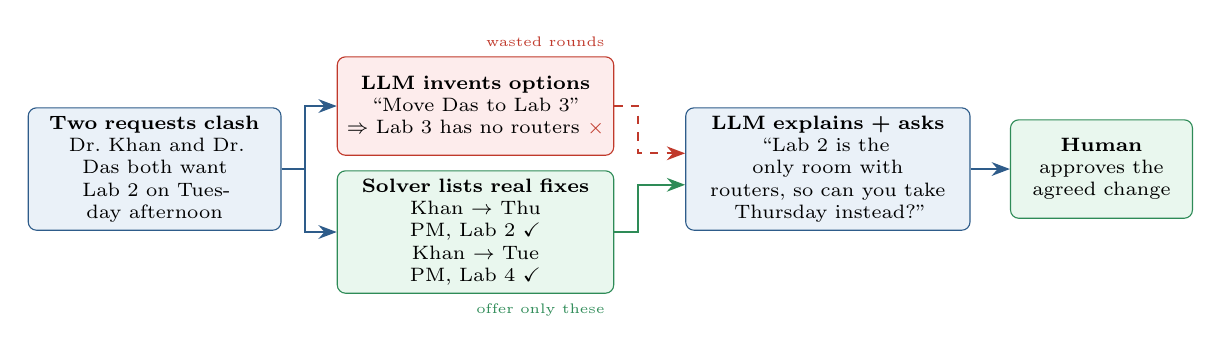
\begin{tikzpicture}[node distance=4mm]
  \node[blk,text width=3.0cm,minimum height=1.25cm] (req)
    {\textbf{Two requests clash}\\Dr.\ Khan and Dr.\ Das both want\\Lab~2 on Tuesday afternoon};
  \node[rblk,text width=3.3cm,minimum height=1.25cm,right=7mm of req,yshift=8mm] (llm)
    {\textbf{LLM invents options}\\``Move Das to Lab~3''\\$\Rightarrow$ Lab~3 has no routers {\color{badred}$\times$}};
  \node[gblk,text width=3.3cm,minimum height=1.25cm,right=7mm of req,yshift=-8mm] (sol)
    {\textbf{Solver lists real fixes}\\Khan $\to$ Thu PM, Lab~2 \checkmark\\Khan $\to$ Tue PM, Lab~4 \checkmark};
  \node[blk,text width=3.4cm,minimum height=1.25cm,right=9mm of sol,yshift=8mm] (talk)
    {\textbf{LLM explains + asks}\\``Lab~2 is the only room with\\routers, so can you take\\Thursday instead?''};
  \node[gblk,text width=2.1cm,minimum height=1.25cm,right=5mm of talk] (ok)
    {\textbf{Human}\\approves the\\agreed change};
  \draw[arr] (req.east) -- ++(3mm,0) |- (llm.west);
  \draw[arr] (req.east) -- ++(3mm,0) |- (sol.west);
  \draw[arr,draw=badred,dashed] (llm.east) -- ++(3mm,0) |- ([yshift=2mm]talk.west);
  \draw[arr,draw=goodgreen] (sol.east) -- ++(3mm,0) |- ([yshift=-2mm]talk.west);
  \node[font=\tiny,text=badred,above=0pt of llm.north east,anchor=south east] {wasted rounds};
  \node[font=\tiny,text=goodgreen,below=0pt of sol.south east,anchor=north east] {offer only these};
  \draw[arr] (talk) -- (ok);
\end{tikzpicture}
\caption{The idea in one picture. Instead of letting the LLM imagine options (red), the solver
lists every minimal valid fix (green) and the LLM only explains and negotiates them.}
\label{fig:teaser}
\end{figure}

\begin{keybox}
\textbf{Research question.} Can solver-derived conflict sets constrain an LLM
negotiator so that it resolves infeasible timetable requests with
\emph{fewer rounds} and \emph{less disruption} than LLM-invented options,
even when those options are filtered by the same solver?
\end{keybox}

\textbf{Hypotheses.} \textbf{H1}: invented options are often invalid and cost
extra rounds or calls. \textbf{H2}: our system resolves at least as often as
generate-and-filter, with fewer rounds, less disruption and a smaller gap to
an all-knowing oracle. \textbf{H3}: explanations tied to solver evidence are
more faithful and leak no private reasons. \textbf{H4}: a concession ledger
spreads the burden of giving way more evenly.

\textbf{Contributions.} (1)~A full working system, from a chat message to a
human-approved timetable, in a web app with role-based views. (2)~A
negotiation benchmark with hidden stakeholder flexibility and a solver
oracle. (3)~Small local fine-tuned models (Qwen3.5-4B + LoRA) for reading
requests, policy checks, reply handling and a tool-calling agent. (4)~A
fairness stress test for the ledger. (5)~An honest report of what did
\emph{not} work.

% ==================================================================
\section{Literature Review}
% ==================================================================
Figure~\ref{fig:lit} places our work among five lines of research.

\textbf{Automated timetabling.} Timetabling has been studied for decades with
local search, integer programming and constraint programming \citep{schaerf1999survey};
the ITC-2007 competition set standard course-timetabling benchmarks \citep{mccollum2010itc}.
Repairing a published timetable with few changes is the \emph{minimal perturbation
problem} \citep{muller2005mpp}. These methods need fully formal constraints; they
cannot read a teacher's message or negotiate. We use OR-Tools CP-SAT \citep{ortools}
for minimal-change repair.

\textbf{Explaining infeasibility.} When a model has no solution, a
\emph{minimal unsatisfiable subset} (MUS) says where the conflict is, and a
\emph{minimal correction set} (MCS) says what could be dropped to fix it
\citep{liffiton2008mus}; MARCO \citep{liffiton2016marco} enumerates them efficiently.
Prior work uses them to help \emph{one} modeller debug a model. We use MCSs as the
\emph{menu of concessions} in a multi-person negotiation.

\textbf{LLMs with solvers.} LLMs plan poorly under hard constraints
\citep{kambhampati2024llmmodulo}. One line of work turns text into optimisation
models \citep{ahmaditeshnizi2024optimus}; another lets the LLM propose and an
external verifier check (``LLM-Modulo'' \citep{kambhampati2024llmmodulo}). In both,
the candidates still come from the LLM. Our B4 baseline is exactly this
generate-and-filter design; we flip it so the solver produces the candidates.

\textbf{LLM negotiation and agents.} Negotiation dialogue can be learned end to
end \citep{lewis2017deal}, and tool-using agents act through typed calls
\citep{yao2023react}. Neither has a model of what is feasible; our agent negotiates
only over solver-verified options.

\textbf{Making small models useful.} LoRA \citep{hu2022lora} and DPO
\citep{rafailov2023dpo} adapt small open models such as Qwen \citep{qwen3} cheaply,
and retrieval-augmented generation (RAG) \citep{lewis2020rag} grounds answers in
documents. For evaluation we use an LLM judge \citep{zheng2023judging} checked
against human labels.

\begin{figure}[H]
\centering
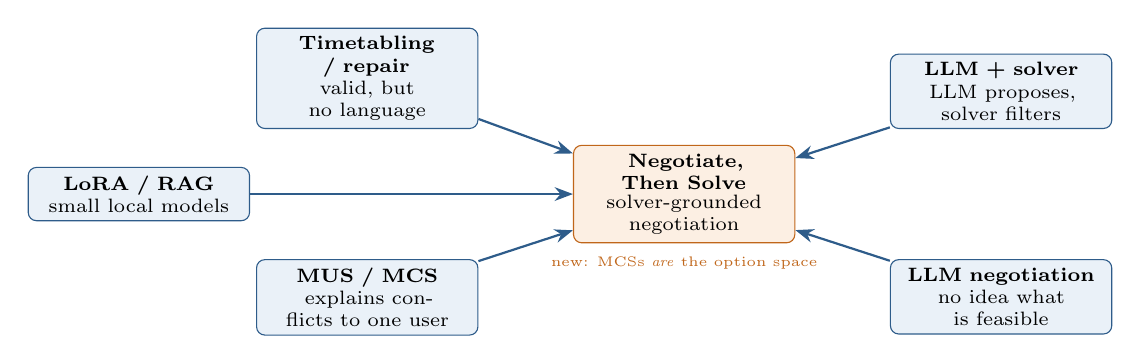
\begin{tikzpicture}
  \node[oblk,text width=2.6cm,minimum height=1.05cm,font=\scriptsize\bfseries] (us)
    {Negotiate, Then Solve\\[-1pt]{\normalfont solver-grounded negotiation}};
  \node[blk,text width=2.6cm,above left=2mm and 12mm of us] (t)
    {\textbf{Timetabling / repair}\\valid, but no language};
  \node[blk,text width=2.6cm,below left=2mm and 12mm of us] (m)
    {\textbf{MUS / MCS}\\explains conflicts to one user};
  \node[blk,text width=2.6cm,above right=2mm and 12mm of us] (l)
    {\textbf{LLM + solver}\\LLM proposes, solver filters};
  \node[blk,text width=2.6cm,below right=2mm and 12mm of us] (n)
    {\textbf{LLM negotiation}\\no idea what is feasible};
  \node[blk,text width=2.6cm,left=12mm of us,xshift=-2.9cm] (f)
    {\textbf{LoRA / RAG}\\small local models};
  \foreach \x/\lab in {t/{repair},m/{conflict sets},l/{verification},n/{dialogue}}
    \draw[arr] (\x) -- (us);
  \draw[arr] (f.east) -- ++(4mm,0) |- (us.west);
  \node[font=\tiny,text=gaporange,below=0.5mm of us,align=center]
    {new: MCSs \emph{are} the option space};
\end{tikzpicture}
\caption{Where our work sits: we combine pieces that existed separately.}
\label{fig:lit}
\end{figure}

% ==================================================================
\section{Datasets Created and Used}
% ==================================================================
No real staff data was used: every dataset is \emph{synthetic or written by
the team}, so the right answer is known by construction. The institute's
real course-offering document was used only to build a realistic demo
department. Table~\ref{tab:data} lists the datasets and Figure~\ref{fig:datamix}
shows how the reading data is mixed.

\begin{table}[!t]
\centering\small
\rowcolors{2}{white}{greyfill}\begin{tabularx}{\textwidth}{L{3.2cm} Y L{2.9cm}}
\arrayrulecolor{secblue}\toprule\arrayrulecolor{black}
\hdr \hd{Dataset} & \hd{What it is and how we made it} & \hd{Size}\\
\arrayrulecolor{secblue}\midrule\arrayrulecolor{black}
Department world & Seeded synthetic CSE department: 30 faculty, 10 student groups, 20 rooms, 5 days $\times$ 8 slots & 202 class sessions\\
A.\ Negotiation & Planted conflicts of 7 kinds (room contention, policy clash, capacity squeeze, deadlock\,\dots); each stakeholder has \emph{hidden} flexibility; a solver oracle gives the best outcome & 60 scenarios (+30 hard)\\
B.\ Requests & Messages generated from known target constraints, then paraphrased, made vague, unauthorised or adversarial; split by template so test wordings are unseen & 600 (400/49/151)\\
Intent data & Requests $\to$ typed intent JSON (17 kinds: move, limit, relate, choices\,\dots); frozen test split + 26 held-out ``suites'' & 4{,}623 / 373 / 417\\
C.\ Policy (RAG) & Synthetic handbook (16 rules) + 4 circulars as PDF, image and HTML; questions with gold rule IDs; 20 questions no rule covers & 109 + 40 + 20\\
D.\ Replies & Stakeholder replies (accept, partial, counter-offer, vague, refusal, injection) with the right tool call & 100\\
Safety set & Authority violations, prompt injections, requests for private reasons & 50\\
Agent data & 49 request families; trajectories collected with Gemini and kept only if verified; DPO pairs from good vs bad runs & 1{,}082 SFT / 541 DPO\\
Head-to-head & Real-style chat queries on the demo department & 41\\
\arrayrulecolor{secblue}\bottomrule\arrayrulecolor{black}
\end{tabularx}
\caption{Datasets. All are synthetic or team-authored with known ground truth.}
\label{tab:data}
\end{table}

\begin{figure}[H]
\centering
\begin{minipage}[c]{0.50\textwidth}
\centering
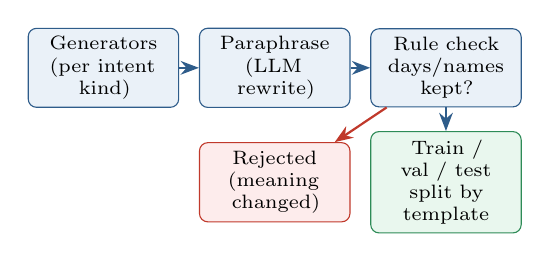
\begin{tikzpicture}[node distance=2.5mm]
  \node[blk,text width=1.7cm] (g) {Generators\\(per intent kind)};
  \node[blk,text width=1.7cm,right=of g] (p) {Paraphrase\\(LLM rewrite)};
  \node[blk,text width=1.7cm,right=of p] (c) {Rule check\\days/names kept?};
  \node[gblk,text width=1.7cm,below=3mm of c] (d) {Train / val / test\\split by template};
  \node[rblk,text width=1.7cm,left=of d] (r) {Rejected\\(meaning changed)};
  \draw[arr] (g) -- (p); \draw[arr] (p) -- (c); \draw[arr] (c) -- (d);
  \draw[arr,draw=badred] (c) -- (r);
\end{tikzpicture}
\end{minipage}%
\begin{minipage}[c]{0.48\textwidth}
\centering
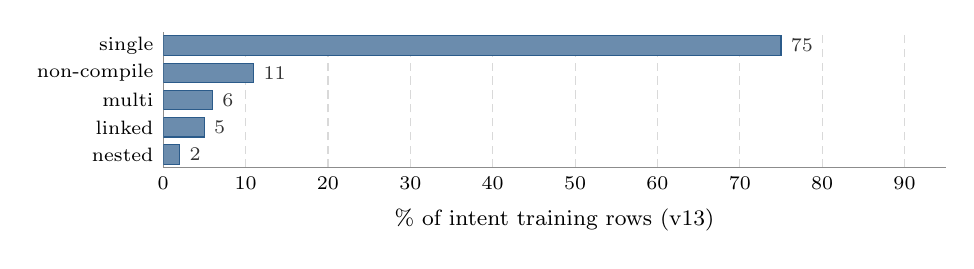
\begin{tikzpicture}
\begin{axis}[nts hbars, width=0.95\linewidth, height=3.3cm, xmax=95,
  symbolic y coords={nested,linked,multi,non-compile,single}, ytick={nested,linked,multi,non-compile,single},
  xlabel={\% of intent training rows (v13)}]
\addplot[fill=secblue!70,draw=secblue] coordinates
  {(75,single) (11,non-compile) (6,multi) (5,linked) (2,nested)};
\end{axis}
\end{tikzpicture}
\end{minipage}
\caption{Left: how request data is made. Right: the training mix is mostly single requests,
which later turned out to be a cause of weak compositional reading (Section~\ref{sec:runs}).}
\label{fig:datamix}
\end{figure}

% ==================================================================
\section{Methodology}
% ==================================================================
\subsection{System overview}
Figure~\ref{fig:arch} follows one request through six steps. Only the
orange step is new research; the rest makes the system real and safe.

\begin{figure}[H]
\centering
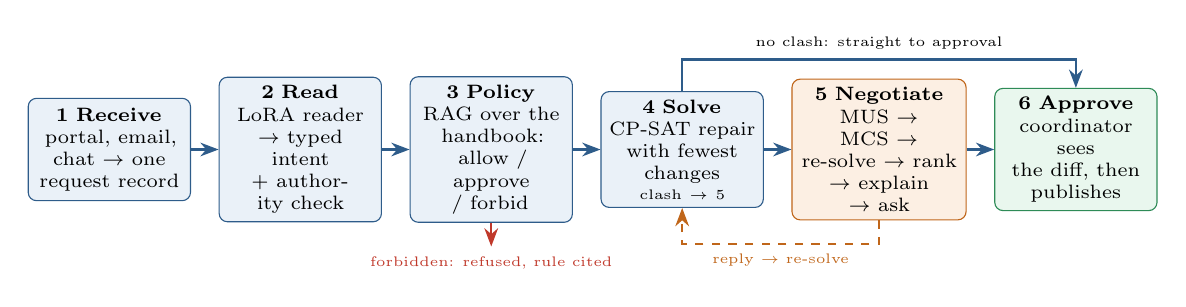
\begin{tikzpicture}[node distance=3.5mm]
  \node[blk,text width=1.85cm,minimum height=1.3cm] (s1) {\textbf{1 Receive}\\portal, email,\\chat $\to$ one\\request record};
  \node[blk,text width=1.85cm,minimum height=1.3cm,right=of s1] (s2) {\textbf{2 Read}\\LoRA reader\\$\to$ typed intent\\+ authority check};
  \node[blk,text width=1.85cm,minimum height=1.3cm,right=of s2] (s3) {\textbf{3 Policy}\\RAG over the\\handbook: allow /\\approve / forbid};
  \node[blk,text width=1.85cm,minimum height=1.3cm,right=of s3] (s4) {\textbf{4 Solve}\\CP-SAT repair\\with fewest\\changes\\[-1pt]{\tiny clash $\to$ 5}};
  \node[oblk,text width=2.0cm,minimum height=1.3cm,right=of s4] (s5) {\textbf{5 Negotiate}\\MUS $\to$ MCS $\to$\\re-solve $\to$ rank\\$\to$ explain $\to$ ask};
  \node[gblk,text width=1.85cm,minimum height=1.3cm,right=of s5] (s6) {\textbf{6 Approve}\\coordinator sees\\the diff, then\\publishes};
  \draw[arr] (s1) -- (s2); \draw[arr] (s2) -- (s3); \draw[arr] (s3) -- (s4);
  \draw[arr] (s4) -- (s5); \draw[arr] (s5) -- (s6);
  \draw[arr] (s4.north) -- ++(0,4mm) -| node[pos=0.25,above,font=\tiny]{no clash: straight to approval} (s6.north);
  \draw[arr,draw=badred] (s3.south) -- ++(0,-3mm) node[below,font=\tiny,text=badred]{forbidden: refused, rule cited};
  \draw[fb] (s5.south) -- ++(0,-3mm) -| node[pos=0.25,below,font=\tiny,text=gaporange]{reply $\to$ re-solve} (s4.south);
\end{tikzpicture}
\caption{Architecture. Every LLM output is a \emph{proposal}: it passes schema, authority,
policy and solver checks, and finally a human, before anything changes.}
\label{fig:arch}
\end{figure}

\subsection{The core idea: solver-grounded negotiation}
Each class gets one slot and one room, subject to room capacity, no
double-booking, teacher availability, student clashes and institute rules.
Each request becomes a constraint $C_i$ guarded by a switch $a_i$
($a_i \Rightarrow C_i$), so the solver can turn requests on and off.
Figure~\ref{fig:core} shows what happens when there is no solution.

\begin{figure}[H]
\centering
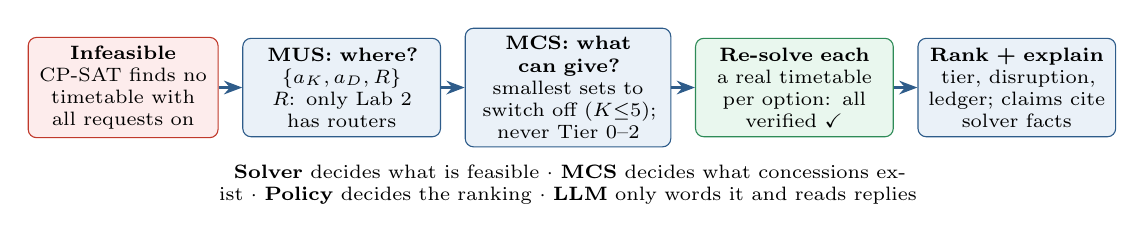
\begin{tikzpicture}[node distance=3mm]
  \node[rblk,text width=2.2cm,minimum height=1.25cm] (a) {\textbf{Infeasible}\\CP-SAT finds no\\timetable with\\all requests on};
  \node[blk,text width=2.3cm,minimum height=1.25cm,right=of a] (b) {\textbf{MUS: where?}\\$\{a_K, a_D, R\}$\\$R$: only Lab~2\\has routers};
  \node[blk,text width=2.4cm,minimum height=1.25cm,right=of b] (c) {\textbf{MCS: what can give?}\\smallest sets to\\switch off ($K{\le}5$);\\never Tier 0--2};
  \node[gblk,text width=2.3cm,minimum height=1.25cm,right=of c] (d) {\textbf{Re-solve each}\\a real timetable\\per option: all\\verified \checkmark};
  \node[blk,text width=2.3cm,minimum height=1.25cm,right=of d] (e) {\textbf{Rank + explain}\\tier, disruption,\\ledger; claims cite\\solver facts};
  \draw[arr] (a)--(b); \draw[arr] (b)--(c); \draw[arr] (c)--(d); \draw[arr] (d)--(e);
  \node[font=\scriptsize,below=1mm of c,text width=12cm,align=center] (who)
    {\textbf{Solver} decides what is feasible $\cdot$ \textbf{MCS} decides what concessions exist
     $\cdot$ \textbf{Policy} decides the ranking $\cdot$ \textbf{LLM} only words it and reads replies};
\end{tikzpicture}
\caption{The negotiation loop. The LLM never adds an option, so no infeasible option can ever be shown.}
\label{fig:core}
\end{figure}

\textbf{Priority tiers.} Constraints sit in six published tiers: T0 physical
(never relaxed), T1 institute policy (Dean), T2 commitments such as exam
blocks (office), and negotiable T3 unavailability, T4 operational needs and
T5 preferences. \textbf{Resolution ladder:} try a free substitute; else
re-solve the 5 cheapest MCSs; rank them; ask the owner with the lowest
burden; turn the reply into a constraint and re-solve; escalate on deadlock,
timeout or any T1--T2 option. \textbf{Concession ledger:} each time someone
gives way they earn credit $1{-}0.5^{c}$ ($c$: weighted concessions so far), which makes them
more expensive to ask next time; each further concession still adds to it.

\subsection{Language components and models}
\begin{figure}[!t]
\centering
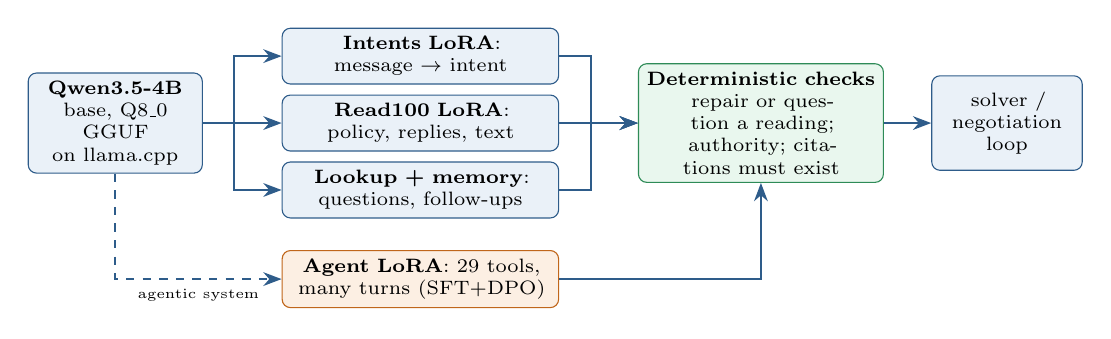
\begin{tikzpicture}[node distance=3mm]
  \node[blk,text width=2.0cm,minimum height=1.2cm] (base) {\textbf{Qwen3.5-4B}\\base, Q8\_0 GGUF\\on llama.cpp};
  \node[blk,text width=3.3cm,right=10mm of base,yshift=8.5mm] (i) {\textbf{Intents LoRA}: message $\to$ intent};
  \node[blk,text width=3.3cm,right=10mm of base] (r) {\textbf{Read100 LoRA}: policy, replies, text};
  \node[blk,text width=3.3cm,right=10mm of base,yshift=-8.5mm] (lk) {\textbf{Lookup + memory}: questions, follow-ups};
  \node[oblk,text width=3.3cm,below=4mm of lk] (ag) {\textbf{Agent LoRA}: 29 tools, many turns (SFT+DPO)};
  \node[gblk,text width=2.9cm,minimum height=1.2cm,right=10mm of r] (chk) {\textbf{Deterministic checks}\\repair or question a reading;\\authority; citations must exist};
  \node[blk,text width=1.7cm,minimum height=1.2cm,right=6mm of chk] (out) {solver /\\negotiation\\loop};
  \draw[arr] (base.east) -- ++(4mm,0) |- (i.west);
  \draw[arr] (base.east) -- (r.west);
  \draw[arr] (base.east) -- ++(4mm,0) |- (lk.west);
  \draw[arr,dashed] (base.south) |- node[pos=0.75,below,font=\tiny]{agentic system} (ag.west);
  \draw[arr] (i.east) -- ++(4mm,0) |- (chk.west);
  \draw[arr] (r.east) -- (chk.west);
  \draw[arr] (lk.east) -- ++(4mm,0) |- (chk.west);
  \draw[arr] (ag.east) -| (chk.south);
  \draw[arr] (chk) -- (out);
\end{tikzpicture}
\caption{One small base model, one LoRA adapter per task group, swapped per request on one
llama.cpp server. Every output goes through rule-based checks.}
\label{fig:models}
\end{figure}

We built \textbf{two final systems} on the same core. The \emph{fine-tuned
pipeline} reads each message with the intents adapter into a typed intent
(17 kinds, Table~\ref{tab:intents}, including limits like ``at most two days a week'' and choices like
``Tuesday, failing that Thursday''); a deterministic compiler turns it into
solver constraints. For example, ``\emph{pls shift my DBMS lec frm monday to thursday
afternoon if possible}'' is read as: move the Monday Database Systems lecture to Thursday
afternoon, as a wish, not a must. The model copies days and names as written and never
writes slot numbers or IDs; code finds the real class, checks the sender may ask, and
sets the tier. The \emph{agentic} system gives a tool-calling agent 29
tools in 8 groups (Table~\ref{tab:tools}) and lets it work a request over many turns. The policy agent retrieves
the top 8 rules with hybrid BM25 + dense search; a denial without a valid
citation is downgraded to ``needs approval'', so nothing is refused without
naming the rule.

\begin{table}[H]
\centering\footnotesize
\renewcommand{\arraystretch}{1.3}
\setlength{\tabcolsep}{5pt}
\begin{tabularx}{\textwidth}{l p{6.3cm} X}
\arrayrulecolor{secblue}\toprule\arrayrulecolor{black}
\hdr \hd{Group} & \hd{Intent kinds (times used in training)} & \hd{Example message}\\
\arrayrulecolor{secblue}\midrule\arrayrulecolor{black}
\textbf{\textcolor{secblue}{Times}} & \texttt{avoid} 891, \texttt{unavailable} 814, \texttt{only} 411 & ``No classes before 10, please''; ``I'm away on Tuesday''\\
\textbf{\textcolor{secblue}{One class}} & \texttt{move} 1{,}044, \texttt{cancel} 322, \texttt{extra\_class} 88, \texttt{swap} 75 & ``Shift my DBMS lecture to Thursday afternoon''\\
\textbf{\textcolor{secblue}{Rooms}} & \texttt{club\_booking} 207, \texttt{needs\_room} 68, \texttt{room\_closed} 40 & ``Our practical needs the lab with GPUs''\\
\textbf{\textcolor{secblue}{Shape of week}} & \texttt{relate} 249, \texttt{load\_limit} 178, \texttt{limit} 148 & ``At most two teaching days a week''; ``not right after the lab''\\
\textbf{\textcolor{secblue}{Choices}} & \texttt{any\_of} 49, \texttt{ranked} 42, \texttt{fallback} 23 & ``Ideally Friday, otherwise Thursday''\\
\textbf{\textcolor{secblue}{Reports}} & \texttt{clash\_report} 139 & ``Two of our classes are both on Monday at 10''\\
\arrayrulecolor{black!25}\midrule\arrayrulecolor{black}
\textbf{\textcolor{secblue}{Action}} & \texttt{compile} 4{,}097, \texttt{clarify} 181, \texttt{investigate} 139, \texttt{out\_of\_scope} 80, \texttt{withdraw} 65, \texttt{answer} 61 & What to do with the message as a whole\\
\arrayrulecolor{secblue}\bottomrule\arrayrulecolor{black}
\end{tabularx}
\caption{What the request reader can write: 17 intent kinds and 6 actions, with how often each appears in the
4{,}623 training messages. Choices wrap other intents, so one message can hold several.}
\label{tab:intents}
\end{table}

\begin{table}[H]
\centering\footnotesize
\renewcommand{\arraystretch}{1.3}
\setlength{\tabcolsep}{5pt}
\begin{tabularx}{\textwidth}{l X r}
\arrayrulecolor{secblue}\toprule\arrayrulecolor{black}
\hdr \hd{Group} & \hd{Tools (calls in the agent's training data)} & \hd{Calls}\\
\arrayrulecolor{secblue}\midrule\arrayrulecolor{black}
\textbf{\textcolor{secblue}{Read}} & \texttt{classes\_of} 518, \texttt{find} 239, \texttt{describe} 59, \texttt{free\_hours} 57, \texttt{who\_is\_free} 25, \texttt{free\_rooms} 2, \texttt{changes} 0 & 900\\
\textbf{\textcolor{secblue}{Policy}} & \texttt{rules} 72: look up and cite the handbook & 72\\
\textbf{\textcolor{secblue}{Draft}} & \texttt{move\_class} 401, \texttt{constrain} 395, \texttt{retract} 146, \texttt{swap\_classes} 93, \texttt{list\_draft} 2 & 1{,}037\\
\textbf{\textcolor{secblue}{Extend}} & \texttt{cancel\_class} 38, \texttt{limit\_hours} 1, \texttt{add\_class} 0, \texttt{book\_room} 0 & 39\\
\textbf{\textcolor{secblue}{Compose}} & \texttt{move\_to\_window} 150, \texttt{limit\_load} 84, \texttt{relate\_classes} 76, \texttt{set\_weeks} 43, \texttt{choose} 41 & 394\\
\textbf{\textcolor{secblue}{Evaluate}} & \texttt{check\_draft} 997: the solver says whether the draft works and who it affects & 997\\
\textbf{\textcolor{secblue}{Talk}} & \texttt{make\_offer} 157, \texttt{ask\_requester} 102, \texttt{message\_party} 4 & 263\\
\textbf{\textcolor{secblue}{End}} & \texttt{submit} 782 (only after \texttt{check\_draft} said ok), \texttt{decline} 111, \texttt{escalate} 56 & 949\\
\arrayrulecolor{secblue}\bottomrule\arrayrulecolor{black}
\end{tabularx}
\caption{The coordinator agent's 29 tools, with their calls in its 1{,}082 training trajectories (4{,}651 in all).
Only \texttt{submit} can change the timetable, and only after the solver has checked the draft.}
\label{tab:tools}
\end{table}

\textbf{Safety boundary.} Messages are treated as data, never instructions.
Every action goes \emph{schema check $\to$ policy + authority $\to$ CP-SAT
$\to$ human approval}. This is code, not a prompt, so even a fully
compromised model cannot publish a change.

\textbf{Training.} Figure~\ref{fig:train} shows the training loop. All
adapters were trained on free Kaggle T4 GPUs across two accounts.
\textbf{Which layers, and why.} Each adapter is rank 16 on the attention projections,
which help the model \emph{find and copy} the right words from the prompt, and on the MLP
projections, which help it \emph{turn} phrases into our formats: about 21M weights, 0.5\% of
the model. Qwen3.5 has 32 layers, but only every fourth uses full attention; the other 24 use
linear attention, whose projections our module pattern missed by accident, so only their
MLPs were trained. We freeze the embeddings and output layer: we need no new words, and
training them would make each adapter over a gigabyte. Full fine-tuning would not fit on
two 15\,GB T4s. Table~\ref{tab:train} gives the other settings.

\begin{figure}[H]
\centering
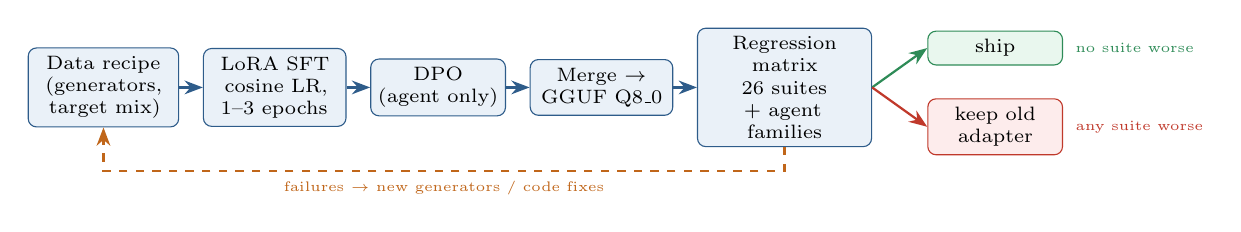
\begin{tikzpicture}[node distance=3mm]
  \node[blk,text width=1.7cm] (d) {Data recipe\\(generators,\\target mix)};
  \node[blk,text width=1.6cm,right=of d] (s) {LoRA SFT\\cosine LR,\\1--3 epochs};
  \node[blk,text width=1.5cm,right=of s] (p) {DPO\\(agent only)};
  \node[blk,text width=1.6cm,right=of p] (g) {Merge $\to$\\GGUF Q8\_0};
  \node[blk,text width=2.0cm,right=of g] (e) {Regression matrix\\26 suites + agent\\families};
  \node[gblk,text width=1.5cm,right=7mm of e,yshift=5mm] (y) {ship};
  \node[rblk,text width=1.5cm,right=7mm of e,yshift=-5mm] (n) {keep old\\adapter};
  \draw[arr] (d)--(s); \draw[arr] (s)--(p); \draw[arr] (p)--(g); \draw[arr] (g)--(e);
  \draw[arr,draw=goodgreen] (e.east) -- (y.west);
  \draw[arr,draw=badred] (e.east) -- (n.west);
  \node[font=\tiny,text=goodgreen,right=1pt of y] {no suite worse};
  \node[font=\tiny,text=badred,right=1pt of n] {any suite worse};
  \draw[fb] (e.south) -- ++(0,-3mm) -| node[pos=0.25,below,font=\tiny,text=gaporange]{failures $\to$ new generators / code fixes} (d.south);
\end{tikzpicture}
\caption{Training loop with a \emph{release rule}: a new adapter ships only if no held-out suite gets worse.}
\label{fig:train}
\end{figure}

\begin{table}[H]
\centering\footnotesize
\rowcolors{2}{white}{greyfill}\begin{tabularx}{\textwidth}{l l Y}
\arrayrulecolor{secblue}\toprule\arrayrulecolor{black}
\hdr \hd{Setting} & \hd{Value} & \hd{Why}\\
\arrayrulecolor{secblue}\midrule\arrayrulecolor{black}
What is learned & Loss on the answer only, not the prompt & The prompt holds one department's details; learning it would memorise them\\
Learning rate & $2{\times}10^{-4}$ new; $5{\times}10^{-5}$ when continuing & A lower rate adjusts what the last version knows instead of overwriting it\\
Number format & fp16 (request reader); fp32 (lookup, memory) & T4s lack bf16; fp16 is much faster but failed in one training stack\\
Passes over data & 3 (request reader); 1 (lookup, memory) & More passes memorise wordings; the reader's rarest skills appear only in pass 3\\
\arrayrulecolor{secblue}\bottomrule\arrayrulecolor{black}
\end{tabularx}
\caption{Training settings. No real user's messages were used.}
\label{tab:train}
\end{table}

% ==================================================================
\section{Experiment Runs}
\label{sec:runs}
% ==================================================================
\textbf{Main experiment setup.} Ours, B3 and B4 each ran the 60 scenarios
$\times$ 3 seeds (180 paired runs). Four stakeholder simulator families
(strict, flexible, cost-sensitive, history-sensitive) hide their true
flexibility; rules decide acceptance and a separate LLM only words the reply.
CP-SAT is single-threaded with a fixed seed, so paired systems see identical
options. Ours used the local 4B; the baselines used the larger Gemini 3.5
Flash-Lite so they were not handicapped on language.

\begin{table}[H]
\centering\small
\rowcolors{2}{white}{greyfill}\begin{tabularx}{\textwidth}{l Y l}
\arrayrulecolor{secblue}\toprule\arrayrulecolor{black}
\hdr \hd{System} & \hd{How it works} & \hd{What it tests}\\
\arrayrulecolor{secblue}\midrule\arrayrulecolor{black}
B1 LLM-only & LLM writes the new timetable directly, no solver & Do we need a solver?\\
B2 Solver-only & Imposes the best repair without asking anyone & Do we need negotiation?\\
B3 Unverified & LLM invents options and offers them unchecked & Cost of invalid options\\
\textbf{B4 Filtered} & LLM invents options; CP-SAT filters; up to 3 regenerations & \textbf{Grounding (main RQ)}\\
\oursrow\textbf{Ours} & Options only from re-solved MCS relaxations & The method under test\\
Oracle & Solver that knows everyone's hidden flexibility & Best possible\\
\arrayrulecolor{secblue}\bottomrule\arrayrulecolor{black}
\end{tabularx}
\caption{Baselines. B4 differs from ours \emph{only} in where the options come from.}
\end{table}

% ==================================================================
\section{Evaluations}
% ==================================================================
\subsection{Main result: grounding beats generate-and-filter (H1, H2)}\label{sec:main}
\begin{figure}[H]
\centering
\begin{minipage}{0.49\textwidth}
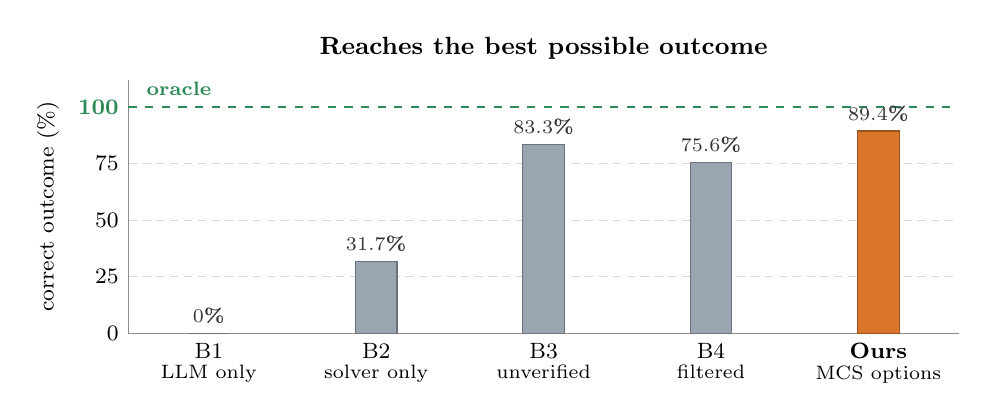
\begin{tikzpicture}
\begin{axis}[nts bars, ymax=112, ytick={0,25,50,75}, ylabel={correct outcome (\%)},
  title={Reaches the best possible outcome},
  xtick={B1,B2,B3,B4,Ours}, symbolic x coords={B1,B2,B3,B4,Ours},
  xticklabels={B1\\[-2pt]{\scriptsize LLM only},B2\\[-2pt]{\scriptsize solver only},B3\\[-2pt]{\scriptsize unverified},B4\\[-2pt]{\scriptsize filtered},\textbf{Ours}\\[-2pt]{\scriptsize MCS options}},
  nodes near coords={\pgfmathprintnumber{\pgfplotspointmeta}\%},
  extra y ticks={100}, extra y tick labels={\textcolor{goodgreen}{\textbf{100}}},
  extra y tick style={grid=major,grid style={dashed,thick,draw=goodgreen}}]
\node[font=\scriptsize\bfseries,text=goodgreen,anchor=south west] at (rel axis cs:0.01,0.90) {oracle};
\addplot[fill=greyb,draw=greyb!70!black] coordinates {(B1,0) (B2,31.7) (B3,83.3) (B4,75.6)};
\addplot[fill=ours,draw=ours!70!black] coordinates {(Ours,89.4)};
\end{axis}
\end{tikzpicture}
\end{minipage}\hfill
\begin{minipage}{0.49\textwidth}
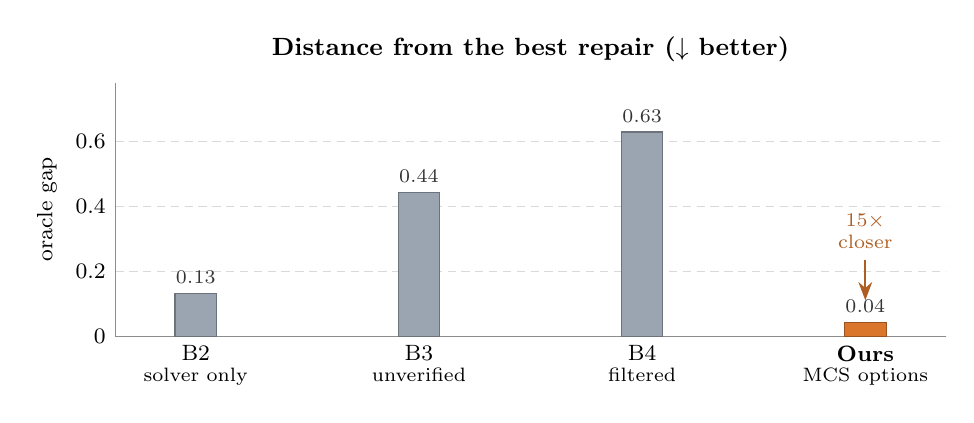
\begin{tikzpicture}
\begin{axis}[nts bars, ymax=0.78, ylabel={oracle gap},
  title={Distance from the best repair ($\downarrow$ better)},
  xtick={B2,B3,B4,Ours}, symbolic x coords={B2,B3,B4,Ours},
  xticklabels={B2\\[-2pt]{\scriptsize solver only},B3\\[-2pt]{\scriptsize unverified},B4\\[-2pt]{\scriptsize filtered},\textbf{Ours}\\[-2pt]{\scriptsize MCS options}},
  yticklabel style={/pgf/number format/fixed}]
\addplot[fill=greyb,draw=greyb!70!black] coordinates {(B2,0.131) (B3,0.443) (B4,0.628)};
\addplot[fill=ours,draw=ours!70!black] coordinates {(Ours,0.041)};
\node[font=\scriptsize,text=ours!80!black,align=center,anchor=south] at (axis cs:Ours,0.24) {15$\times$\\closer};
\draw[->,thick,ours!80!black] (axis cs:Ours,0.235) -- (axis cs:Ours,0.11);
\end{axis}
\end{tikzpicture}
\end{minipage}
\caption{Main experiment (180 paired runs). McNemar: ours vs B4 $p{=}4.6{\times}10^{-6}$, vs B3 $p{=}0.013$.}
\label{fig:main}
\end{figure}

\begin{table}[H]
\centering\footnotesize
\setlength{\tabcolsep}{4pt}
\rowcolors{2}{white}{greyfill}\begin{tabularx}{\textwidth}{l c C C C C C C C c}
\arrayrulecolor{secblue}\toprule\arrayrulecolor{black}
\hdr \hd{System} & \hd{$n$} & \hd{Correct} & \hd{Agreed} & \hd{Escalated} & \hd{Rounds} & \hd{Oracle gap} & \hd{Worse tier} & \hd{LLM calls} & \hd{Invalid options}\\
\arrayrulecolor{secblue}\midrule\arrayrulecolor{black}
B1 LLM-only & 20 & 0.0\% & 0.0\% & 0.0\% & n/a & n/a & n/a & n/a & 80\% of timetables$^{a}$\\
B2 Solver-only & 60 & 31.7\% & 0.0\% & 13.3\% & n/a & 0.131$^{c}$ & 0\% & 0 & 0\\
B3 Unverified & 180 & 83.3\% & 66.7\% & 48.3\% & 1.47 & 0.443 & 35\% & 2.26 & 51.0\%\\
B4 Filtered & 180 & 75.6\% & 51.1\% & 56.1\% & 1.48 & 0.628 & 50\% & 3.97 & 5.7 per scenario$^{b}$\\
\oursrow\textbf{Ours} & 180 & \textbf{89.4\%} & \textbf{78.9\%} & \textbf{42.2\%} & \textbf{1.38} & \textbf{0.041} & \textbf{0\%} & \textbf{0} & \textbf{0}\\
\rowcolor{goodfill}Oracle & 60 & 100\% & 100\% & 31.7\% & 0 & 0 & 0\% & 0 & 0\\
\arrayrulecolor{secblue}\bottomrule\arrayrulecolor{black}
\end{tabularx}
\caption{Main results. \emph{Agreed}: share of the scenarios that can be agreed which end in agreement.
\emph{Escalated}: sent to a human; the oracle's 31.7\% is the floor (those conflicts cannot be agreed).
\emph{Worse tier}: the final repair relaxes a more important constraint than the oracle's.
\emph{LLM calls}: calls per scenario to invent options. n/a: the system does not negotiate.
Differences in rounds are not significant.
$^{a}$timetables that break a hard rule; $^{b}$invented options thrown out by the solver;
$^{c}$absolute gap: imposed repairs are cheap on paper, but only 9.8\% were acceptable to the people affected.}
\end{table}

\begin{takeaway}
\tk{Half of the LLM's invented options are impossible (B3: 51\%). Filtering them (B4)
makes things \emph{worse}, not better: the survivors are few and poor, so B4 agrees less
often than B3, escalates most (56\%), and in half its scenarios ends with a repair that gives up a
more important constraint than needed. Ours never does (0\%), needs no LLM calls to find options,
and its first offer is accepted 28\% of the time against 11--13\% for B3/B4.}
\end{takeaway}

\textbf{Is it just the model?} We re-ran ours and B4 \emph{both} on Gemini (20
scenarios). Ours on Gemini resolved exactly the conflicts ours on the 4B
resolved (7 vs 7; 18/20 identical outcomes); B4 resolved 4 and needed 5.1 LLM
calls per scenario vs 0. The gain comes from the option source, not the model
(this small run alone is not significant, $p{=}0.38$).

\subsection{Capability results}
\begin{figure}[H]
\centering
\begin{minipage}{0.32\textwidth}
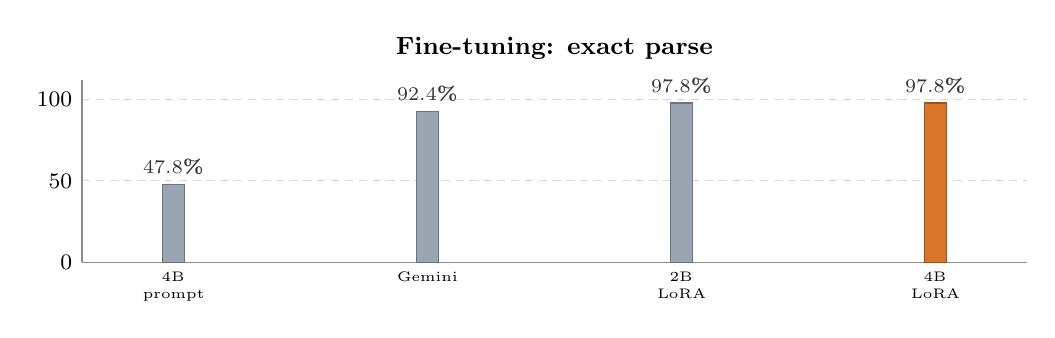
\begin{tikzpicture}
\begin{axis}[nts bars, ymax=112, width=1.12\linewidth, height=3.9cm, bar width=8pt,
  title={Fine-tuning: exact parse},
  nodes near coords={\pgfmathprintnumber{\pgfplotspointmeta}\%}, ytick={0,50,100},
  xtick={4B prompt,Gemini,2B LoRA,4B LoRA}, symbolic x coords={4B prompt,Gemini,2B LoRA,4B LoRA},
  xticklabel style={font=\tiny,align=center,text width=0.9cm}]
\addplot[fill=greyb,draw=greyb!70!black] coordinates {(4B prompt,47.8) (Gemini,92.4) (2B LoRA,97.8)};
\addplot[fill=ours,draw=ours!70!black] coordinates {(4B LoRA,97.8)};
\end{axis}
\end{tikzpicture}
\end{minipage}\hfill
\begin{minipage}{0.32\textwidth}
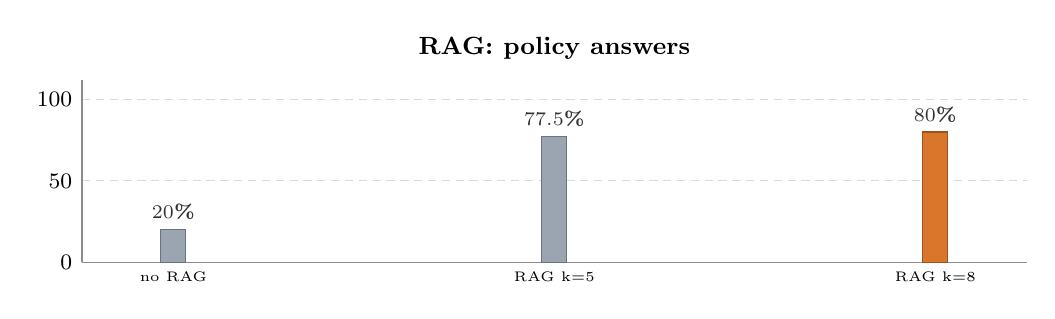
\begin{tikzpicture}
\begin{axis}[nts bars, ymax=112, width=1.12\linewidth, height=3.9cm, bar width=9pt,
  title={RAG: policy answers},
  nodes near coords={\pgfmathprintnumber{\pgfplotspointmeta}\%}, ytick={0,50,100},
  xtick={no RAG,RAG k=5,RAG k=8}, symbolic x coords={no RAG,RAG k=5,RAG k=8},
  xticklabel style={font=\tiny}]
\addplot[fill=greyb,draw=greyb!70!black] coordinates {(no RAG,20.0) (RAG k=5,77.5)};
\addplot[fill=ours,draw=ours!70!black] coordinates {(RAG k=8,80.0)};
\end{axis}
\end{tikzpicture}
\end{minipage}\hfill
\begin{minipage}{0.32\textwidth}
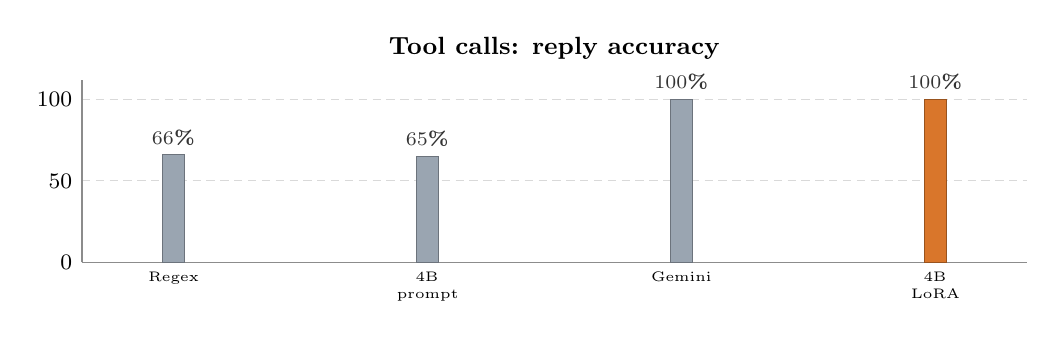
\begin{tikzpicture}
\begin{axis}[nts bars, ymax=112, width=1.12\linewidth, height=3.9cm, bar width=8pt,
  title={Tool calls: reply accuracy},
  nodes near coords={\pgfmathprintnumber{\pgfplotspointmeta}\%}, ytick={0,50,100},
  xtick={Regex,4B prompt,Gemini,4B LoRA}, symbolic x coords={Regex,4B prompt,Gemini,4B LoRA},
  xticklabel style={font=\tiny,align=center,text width=0.9cm}]
\addplot[fill=greyb,draw=greyb!70!black] coordinates {(Regex,66) (4B prompt,65) (Gemini,100)};
\addplot[fill=ours,draw=ours!70!black] coordinates {(4B LoRA,100)};
\end{axis}
\end{tikzpicture}
\end{minipage}
\caption{Each capability against its baseline (\%). Left: 151 unseen requests. Middle: 40
questions worded unlike the rules. Right: 100 replies; the regex handler gets 0\% on counter-offers
and vague replies, and Gemini's tool choice is right but only 85.5\% of its arguments are.}
\label{fig:caps}
\end{figure}

\begin{itemize}
\item \textbf{Fine-tuning.} LoRA lifts the \emph{same} 4B from 47.8\% to 97.8\% exact
compilation at one sixth of the latency (2.0\,s vs 13.2\,s), and beats prompted Gemini.
The deployed intents reader (v12) scores 96.4\% on the frozen test and 95.9\% with typos
or noise; the rule-based parser scores 51.6\%. An encoder reader (DeBERTa started from
GLiNER2) reached 98.1\% on the test split at 83\,ms per message, but is weaker on unseen
wordings (89--91\% vs 95\%), so it is a promising fast path, not a replacement.
\item \textbf{RAG.} Without retrieval the model invents policy (``10 days of casual leave'').
With retrieval it abstains on 100\% of questions no rule covers (vs 75\%), cites 0 fake
rules, and hybrid search at $k{=}8$ finds the right rule 95\% of the time
(Figure~\ref{fig:rag}). On ordinary requests, verdicts are 100\% correct.
\item \textbf{Agentic.} The fine-tuned agent v4 passes 100\% of 19 families (prompted
Gemini 85.1\%, prompted 4B 66.7\%); v6-dpo passes 412/480 episodes over 49 harder families.
In a 41-query head-to-head on the demo, code fixes alone lifted the agent from 28 to 36 and
the pipeline from 35 to 39; the pipeline is also 2--3$\times$ faster (6\,s vs 15\,s median).
\end{itemize}

\begin{figure}[H]
\centering
\begin{minipage}{0.48\textwidth}
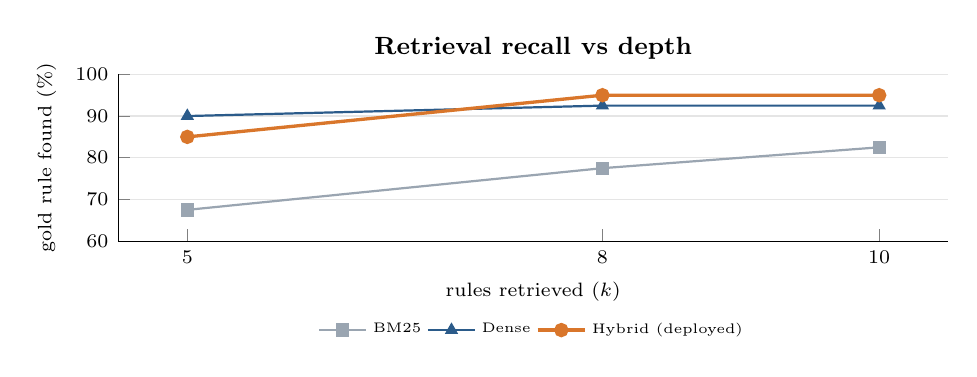
\begin{tikzpicture}
\begin{axis}[width=\linewidth,height=3.7cm, axis lines*=left, ymajorgrids,
  grid style={draw=black!10}, ymin=60, ymax=100, xtick={5,8,10},
  xlabel={rules retrieved ($k$)}, ylabel={gold rule found (\%)},
  tick label style={font=\scriptsize}, label style={font=\scriptsize},
  legend style={font=\tiny,at={(0.5,-0.42)},anchor=north,legend columns=3,draw=none,fill=none},
  title={Retrieval recall vs depth}, title style={font=\small\bfseries,yshift=-4pt}]
\addplot[greyb,mark=square*,thick] coordinates {(5,67.5) (8,77.5) (10,82.5)};
\addplot[secblue,mark=triangle*,thick] coordinates {(5,90) (8,92.5) (10,92.5)};
\addplot[ours,mark=*,very thick] coordinates {(5,85) (8,95) (10,95)};
\legend{BM25,Dense,Hybrid (deployed)}
\end{axis}
\end{tikzpicture}
\end{minipage}\hfill
\begin{minipage}{0.48\textwidth}
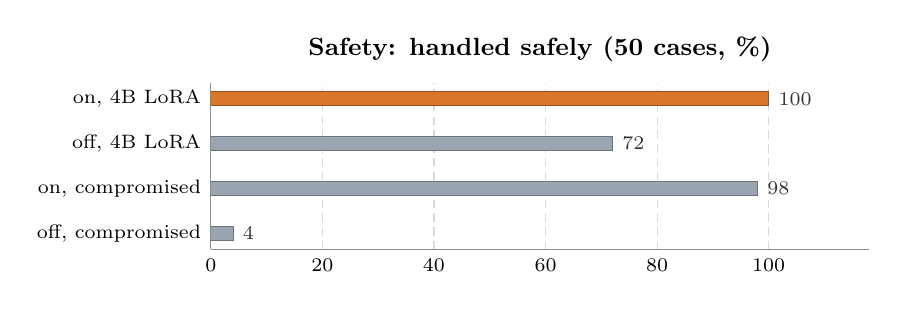
\begin{tikzpicture}
\begin{axis}[nts hbars, width=0.82\linewidth, height=3.7cm, xmax=118, bar width=5pt,
  title={Safety: handled safely (50 cases, \%)},
  bar shift=0pt,
  symbolic y coords={{off, compromised},{on, compromised},{off, 4B LoRA},{on, 4B LoRA}},
  ytick={{off, compromised},{on, compromised},{off, 4B LoRA},{on, 4B LoRA}},
  yticklabel style={font=\scriptsize}]
\addplot[fill=greyb,draw=greyb!70!black] coordinates {(4,{off, compromised}) (98,{on, compromised}) (72,{off, 4B LoRA})};
\addplot[fill=ours,draw=ours!70!black] coordinates {(100,{on, 4B LoRA})};
\end{axis}
\end{tikzpicture}
\end{minipage}
\caption{Left: hybrid search finds the right rule most often. Right: deterministic checks
``on'' vs ``off''. With checks on, even a model that obeys every injection publishes nothing
unapproved; with them off, the good 4B model still lets 14 changes publish unseen.}
\label{fig:rag}
\end{figure}

\subsection{Fairness: does the ledger spread the burden? (H4)}
The benchmark's conflicts are independent one-offs, so the ledger rarely
meets the same person twice. We therefore built a stress test: the same four
teachers, 24 lab clashes per semester, 10 semesters. Two of them (F-301,
F-304) teach the smallest section, so moving them is always ``cheapest'' on paper.

\begin{figure}[H]
\centering
\begin{minipage}{0.40\textwidth}
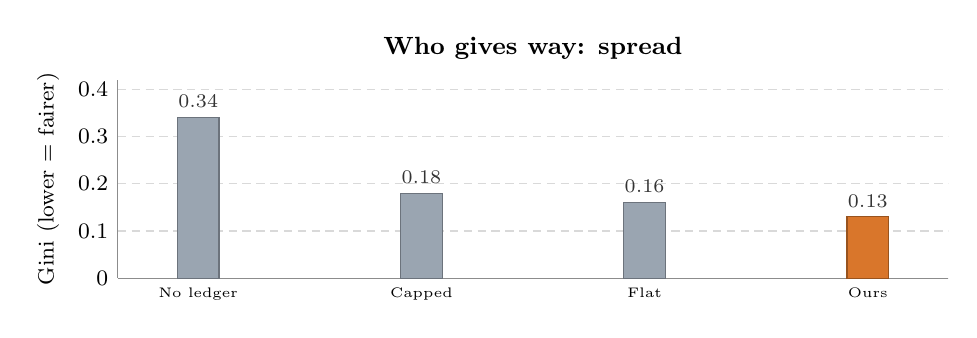
\begin{tikzpicture}
\begin{axis}[nts bars, ymax=0.42, height=4.1cm, ylabel={Gini (lower = fairer)},
  title={Who gives way: spread},
  xtick={No ledger,Capped,Flat,Ours}, symbolic x coords={No ledger,Capped,Flat,Ours},
  xticklabel style={font=\tiny},
  yticklabel style={/pgf/number format/fixed},
  every node near coord/.append style={/pgf/number format/fixed,/pgf/number format/precision=2}]
\addplot[fill=greyb,draw=greyb!70!black] coordinates {(No ledger,0.34) (Capped,0.18) (Flat,0.16)};
\addplot[fill=ours,draw=ours!70!black] coordinates {(Ours,0.13)};
\end{axis}
\end{tikzpicture}
\end{minipage}\hfill
\begin{minipage}{0.57\textwidth}
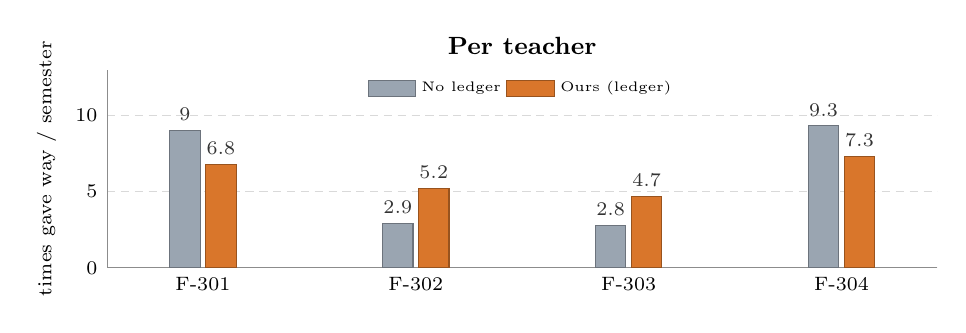
\begin{tikzpicture}
\begin{axis}[ybar, bar width=11pt, ymin=0, ymax=13, height=4.1cm, width=\linewidth,
  axis x line*=bottom, axis y line*=left, ymajorgrids, major tick length=0pt,
  grid style={densely dashed,draw=black!15}, axis line style={draw=black!45},
  symbolic x coords={F-301,F-302,F-303,F-304}, xtick=data,
  ylabel={times gave way / semester}, tick label style={font=\scriptsize},
  label style={font=\scriptsize}, title={Per teacher},
  title style={font=\small\bfseries,yshift=-4pt},
  nodes near coords, every node near coord/.append style={font=\scriptsize\bfseries,text=black!80},
  area legend,
  legend style={font=\tiny,at={(0.5,1.0)},anchor=north,legend columns=2,draw=none,fill=none},
  enlarge x limits=0.15]
\addplot[fill=greyb,draw=greyb!70!black] coordinates {(F-301,9.0) (F-302,2.9) (F-303,2.8) (F-304,9.3)};
\addplot[fill=ours,draw=ours!70!black] coordinates {(F-301,6.8) (F-302,5.2) (F-303,4.7) (F-304,7.3)};
\legend{No ledger, Ours (ledger)}
\end{axis}
\end{tikzpicture}
\end{minipage}
\caption{Fairness stress test (10 semesters, paired Wilcoxon). The ledger cuts the Gini from
0.34 to 0.13 ($p{=}0.002$) and the maximum burden by 3.3, with 100\% of
conflicts still resolved. \emph{Capped}: the earlier credit $\min(1,c)$, which stopped growing after one concession.}
\label{fig:fair}
\end{figure}

\begin{takeaway}
\tk{Without the ledger, the two ``cheap'' teachers give way three times as often as the others.
Flat weights, which ignore tiers and history, come close (0.16, $p{=}0.09$, not significant).
The earlier capped credit was less fair (0.18, $p{=}0.012$), so the live system now uses $1{-}0.5^c$.}
\end{takeaway}

\subsection{Explanations and the human study (H3)}
Grounded explanations name the \emph{constraint}, never the private reason: \textbf{0}
leaks vs \textbf{12} for free text (A2; in 4 of 30 scenarios, so not significant), with first-offer acceptance not lower (4/19 vs 2/19).
Team members, blind to the system, then rated messages and labelled claims. Free text was rated
\emph{more} acceptable (3.77 vs 3.41, 22 paired items, 3 raters, Wilcoxon $p{=}0.019$), with equal
clarity (3.73 vs 3.64, $p{=}0.71$). Humans agreed on claim support only at $\kappa{=}0.39$
($n{=}33$), below our 0.6 bar, so we do not report LLM-judged faithfulness. Other checks passed:
the RAG judge agreed with humans ($\kappa{=}0.72$ and $0.91$), and humans agreed with the reply
tool call in all 40 labelled cases.

\begin{figure}[H]
\centering
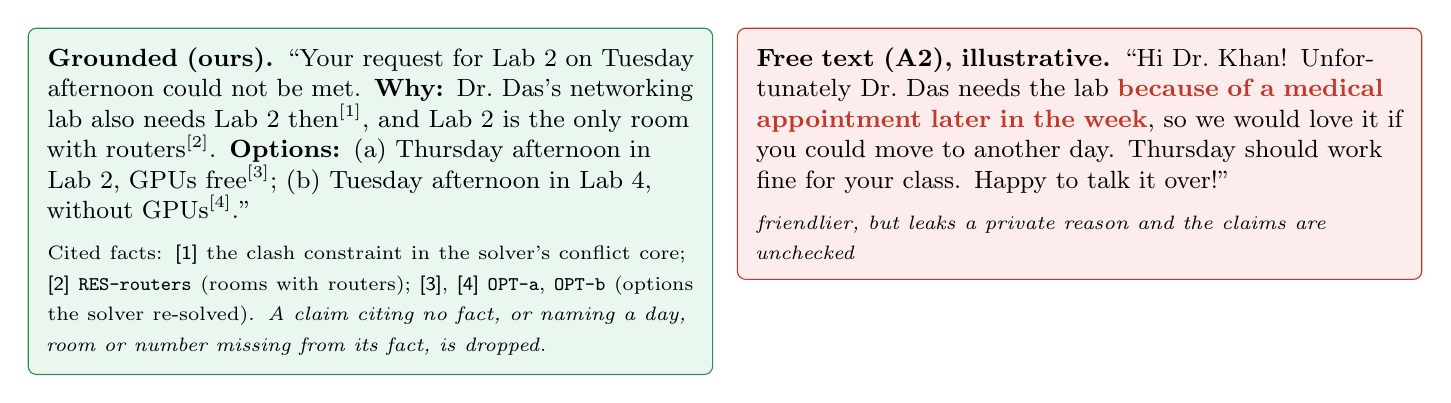
\begin{tikzpicture}
  \node[gblk,text width=8.2cm,align=left,font=\small,inner sep=7pt,anchor=north] (g) at (0,0) {\textbf{Grounded (ours).}
    ``Your request for Lab~2 on Tuesday afternoon could not be met. \textbf{Why:} Dr.\ Das's networking
    lab also needs Lab~2 then$^{[1]}$, and Lab~2 is the only room with routers$^{[2]}$.
    \textbf{Options:} (a) Thursday afternoon in Lab~2, GPUs free$^{[3]}$; (b) Tuesday afternoon in
    Lab~4, without GPUs$^{[4]}$.''\\[4pt]{\scriptsize Cited facts:
    \textsf{[1]} the clash constraint in the solver's conflict core;
    \textsf{[2]} \texttt{RES-routers} (rooms with routers);
    \textsf{[3]}, \textsf{[4]} \texttt{OPT-a}, \texttt{OPT-b} (options the solver re-solved).
    \itshape A claim citing no fact, or naming a day, room or number missing from its fact, is dropped.}};
  \node[rblk,text width=8.2cm,align=left,font=\small,inner sep=7pt,anchor=north west] (f) at ([xshift=3mm]g.north east) {\textbf{Free text (A2), illustrative.}
    ``Hi Dr.\ Khan! Unfortunately Dr.\ Das needs the lab \textcolor{badred}{\textbf{because of a medical appointment
    later in the week}}, so we would love it if you could move to another day. Thursday should work fine for
    your class. Happy to talk it over!''\\[4pt]{\scriptsize\itshape friendlier, but leaks a private reason and the claims are unchecked}};
\end{tikzpicture}
\caption{The same conflict explained two ways. Raters preferred the warmer tone on the right, but
only the left one is safe to send.}
\label{fig:msgs}
\end{figure}

\begin{figure}[H]
\centering
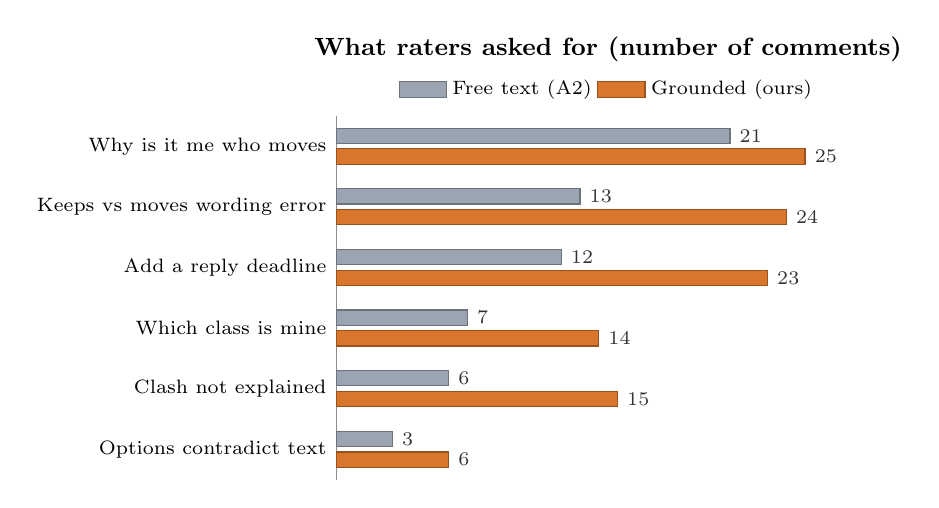
\begin{tikzpicture}
\begin{axis}[nts hbars, width=0.7\textwidth, height=6.2cm, xmax=29, bar width=5.5pt,
  enlarge y limits=0.1, xmajorgrids=false, xtick=\empty, axis x line=none,
  title={What raters asked for (number of comments)}, title style={yshift=12pt},
  ytick=data,
  symbolic y coords={{Options contradict text},{Clash not explained},{Which class is mine},{Add a reply deadline},{Keeps vs moves wording error},{Why is it me who moves}},
  yticklabel style={font=\scriptsize},
  area legend, reverse legend,
  legend style={font=\scriptsize,at={(0.5,1.0)},anchor=south,legend columns=2,draw=none,yshift=2pt}]
\addplot[fill=ours,draw=ours!70!black] coordinates {(25,{Why is it me who moves}) (24,{Keeps vs moves wording error}) (23,{Add a reply deadline}) (14,{Which class is mine}) (15,{Clash not explained}) (6,{Options contradict text})};
\addplot[fill=greyb,draw=greyb!70!black] coordinates {(21,{Why is it me who moves}) (13,{Keeps vs moves wording error}) (12,{Add a reply deadline}) (7,{Which class is mine}) (6,{Clash not explained}) (3,{Options contradict text})};
\legend{Grounded (ours), Free text (A2)}
\end{axis}
\end{tikzpicture}
\caption{Rater feedback themes (73 comments). The biggest gap for both systems: messages do not say why
\emph{this} person was asked. Free text read friendlier, but leaked colleagues' medical appointments.}
\label{fig:study}
\end{figure}

% ==================================================================
\section{Ablations}
% ==================================================================
An ablation changes exactly one thing. Table~\ref{tab:ablsetup} shows what each one swaps out;
Table~\ref{tab:abl} pairs A1--A3 with ours on the same 30 scenarios and seed; Table~\ref{tab:ablall}
covers the rest of the system.

\begin{table}[H]
\centering\footnotesize
\setlength{\tabcolsep}{4pt}
\rowcolors{2}{white}{greyfill}\begin{tabular}{l l l}
\arrayrulecolor{secblue}\toprule\arrayrulecolor{black}
\hdr & \hd{Ablation uses} & \hd{Ours uses}\\
\arrayrulecolor{secblue}\midrule\arrayrulecolor{black}
A1 & flat priorities: every request equal, no ledger & tiers + weights + ledger\\
A2 & free text written from the raw requests (private reasons included) & grounded claims that must cite facts\\
A3 & regex keyword rules to read replies & 4B LoRA tool call\\
\arrayrulecolor{secblue}\bottomrule\arrayrulecolor{black}
\end{tabular}
\caption{The one thing each ablation swaps. Held fixed: solver options, 4B LoRA agent, Gemini
Flash-Lite simulated people, the same 30 scenarios, seed 0. Ablated elsewhere: option source (B3/B4),
ledger credit (Figure~\ref{fig:fair}), retrieval, safety and readers (Table~\ref{tab:ablall}).}
\label{tab:ablsetup}
\end{table}

\begin{table}[H]
\centering\footnotesize
\setlength{\tabcolsep}{4pt}
\rowcolors{2}{white}{greyfill}\begin{tabularx}{\textwidth}{l C C C C C C C C}
\arrayrulecolor{secblue}\toprule\arrayrulecolor{black}
\hdr \hd{30 paired scenarios} & \hd{Resolved} & \hd{Correct} & \hd{Other person gives way} & \hd{Classes moved} & \hd{Options omitted} & \hd{Private leaks} & \hd{1st offer OK} & \hd{Gini}\\
\arrayrulecolor{secblue}\midrule\arrayrulecolor{black}
\oursrow\textbf{Ours} & 10/13 & 27/30 & -- & 2.00 & \textbf{0} & \textbf{0} & \textbf{4/19} & \textbf{0.25}\\
A1 Flat weights & 10/13 & 27/30 & 0/10 & 2.00 & 0 & 0 & 4/19 & 0.25\\
A2 Free-text explanations & 10/13 & 27/30 & 1/10 & 2.06 & 10 & 12 & 2/19 & 0.30\\
A3 Regex reply handler & 10/13 & 27/30 & 1/10 & 2.06 & 0 & 0 & 2/19 & 0.30\\
\arrayrulecolor{secblue}\midrule\arrayrulecolor{black}
\hiderowcolors
\multicolumn{9}{l}{\emph{Current code, all 60 scenarios $\times$ 3 seeds, scripted replies (no LLM):}}\\
\showrowcolors
\oursrow\textbf{Ours} & 85/90 & 175/180 & -- & 1.81 & 0 & 0 & \textbf{29\%} & \textbf{0.149}\\
A1 Flat weights & 84/90 & 174/180 & 2/84 & 1.80 & 0 & 0 & 21\% & 0.154\\
\arrayrulecolor{secblue}\bottomrule\arrayrulecolor{black}
\end{tabularx}
\caption{Each ablation vs ours on the same scenarios. Resolved and Correct match because the simulated
people can only pick from the options offered. \textbf{Top:} no difference is significant; the small changes
are noise. With 3 seeds on the current code, free text (A2) leaks private reasons significantly more
(35 vs 0, $p{=}0.026$). \textbf{Bottom:} without tiers and the ledger (A1), fewer first offers are accepted
(21\% vs 29\%, $p{=}0.002$). \emph{Other person gives way}: a different person conceded than in ours.
\emph{Options omitted}: offered but not mentioned in the message.}
\label{tab:abl}
\end{table}

\textbf{Negotiation.} Outcomes are set by where the options come from, not by A1--A3. The
ledger only matters when the same people meet again (hence the stress test, Figure~\ref{fig:fair}).
Regex replies look fine only because these simulated replies were plain yes/no; on the full reply
set they fail every counter-offer. Free text also left out 10 of the options on offer.

\begin{table}[H]
\centering\footnotesize
\renewcommand{\arraystretch}{1.42}
\setlength{\tabcolsep}{5pt}
\begin{tabularx}{\textwidth}{l p{5.6cm} X}
\arrayrulecolor{secblue}\toprule\arrayrulecolor{black}
\hdr \hd{Part} & \hd{Ablation (one change)} & \hd{Result}\\
\arrayrulecolor{secblue}\midrule\arrayrulecolor{black}
\textbf{\textcolor{secblue}{Negotiation}} & B2: impose the best repair, ask no one & 31.7\% vs \textbf{89.4\%} correct; the most one teacher gives way: 9.19 vs 5.58\\
\arrayrulecolor{black!15}\midrule\arrayrulecolor{black}
\textbf{\textcolor{secblue}{Reading}} & Qwen3.5-2B vs 4B, same data & Same exact parse (97.8\%); right action 96.5 vs \textbf{99.3\%}\\
 & Names looked up by code, not put in the prompt & Prompt 1{,}800 $\to$ 300 chars; training \textbf{7$\times$ cheaper}\\
 & More data generators (v12 $\to$ v13) & Answered 0.68 $\to$ 1.00, but compound 1.00 $\to$ 0.65\\
 & Passes over data (pass 2 vs 3) & Test 0.98 vs 0.96; one rare skill learned only in pass 3\\
\arrayrulecolor{black!15}\midrule\arrayrulecolor{black}
\textbf{\textcolor{secblue}{Rules}} & Search by words / meaning / both (top 5) & 87.7 / 91.5 / \textbf{93.4\%} of rules found\\
\arrayrulecolor{black!15}\midrule\arrayrulecolor{black}
\textbf{\textcolor{secblue}{Safety}} & Checks off vs on, reader obeys every attack & 4\% vs \textbf{98\%} of 50 attack cases safe\\
\arrayrulecolor{black!15}\midrule\arrayrulecolor{black}
\textbf{\textcolor{secblue}{Questions}} & Our department / names shuffled / unseen & 346, 346, 343 of $\sim$360: no memorising\\
 & Output format only (lookup v3.2 vs v4) & Long messages 119 vs \textbf{140} of 200; single questions equal\\
\arrayrulecolor{black!15}\midrule\arrayrulecolor{black}
\textbf{\textcolor{secblue}{Agent}} & Extra DPO step (v7 SFT vs SFT+DPO) & 387 vs 381 of 490 episodes: no gain\\
 & Five tool fixes, no new training & Those request kinds 24 $\to$ \textbf{47} of 50\\
\arrayrulecolor{secblue}\bottomrule\arrayrulecolor{black}
\end{tabularx}
\caption{Ablations across the rest of the system. Each row changes one thing on the same test set.}
\label{tab:ablall}
\end{table}

\begin{takeaway}
\tk{When code can decide, let code decide: checked options beat invented ones, name look-up
made training 7$\times$ cheaper, the checks kept a compromised reader safe, and tool fixes did what
DPO could not. When language must be read, a small model trained on the task wins.}
\end{takeaway}

\begin{table}[H]
\centering\small
\rowcolors{2}{white}{greyfill}\begin{tabularx}{\textwidth}{l Y l}
\arrayrulecolor{secblue}\toprule\arrayrulecolor{black}
\hdr \hd{Hyp.} & \hd{Final evidence} & \hd{Verdict}\\
\arrayrulecolor{secblue}\midrule\arrayrulecolor{black}
H1 & 51\% of B3's options impossible; B4 needs 3.97 LLM calls per scenario and agrees least & \yes{} (rounds n.s.)\\
H2 & Correct 89.4\% vs 75.6\% ($p{=}4.6{\times}10^{-6}$); gap 0.04 vs 0.63; worse tier 0\% vs 50\% & \yes{} (except rounds)\\
H3 & 0 vs 12 leaks; but humans rated free text more acceptable ($p{=}0.019$); claim $\kappa{=}0.39$ & \partly{}\\
H4 & Gini 0.13 vs 0.34 without the ledger ($p{=}0.002$); vs flat 0.16 ($p{=}0.09$) & \yes{} (vs no ledger)\\
\arrayrulecolor{secblue}\bottomrule\arrayrulecolor{black}
\end{tabularx}
\caption{Hypothesis scorecard.}
\end{table}

% ==================================================================
\section{Limitations}
% ==================================================================
\begin{itemize}
\item \textbf{Synthetic world, mixed models.} All data is synthetic and the simulated people are
not real. Ours ran on the 4B and the baselines on Gemini; the same-model check is small ($n{=}20$). The main runs used the earlier capped ledger credit; their
one-off conflicts rarely reach the ledger (A1 changed who gives way in 0 of 10).
\item \textbf{The option space can be too narrow.} 8 of our 19 misses happened because the option
the person would accept was not among the 5 cheapest MCSs; the other 11 were timeouts. Every
miss was a safe escalation, never an invalid timetable.
\item \textbf{Weak human validation.} Raters were team members, not faculty; claim agreement was
low ($\kappa{=}0.39$); the faculty pilot did not happen (no ethics clearance in time).
\item \textbf{Training gaps and compute.} Our LoRA pattern missed the attention of 24 of 32 layers;
continued training forgets what new data leaves out (v13); free T4 GPUs forced bundled retraining.
\end{itemize}

% ==================================================================
\section{Conclusions}
% ==================================================================
\begin{bluebox}{What we learned}
\begin{enumerate}
\item \textbf{Let the solver choose, let the LLM talk.} MCS options reach the best outcome in
89.4\% of runs vs 75.6\% for generate-and-filter, 15$\times$ closer to the best repair, with no
impossible offers; the ledger cuts the unfairness of who gives way from 0.34 to 0.13.
\item \textbf{Small fine-tuned models are enough.} A local 4B with LoRA beat a large prompted
model at reading requests (97.8\% vs 92.4\%), so private staff data never leaves the institute.
\item \textbf{Safety lives in code, not prompts.} Checks and approval kept 98\% of attacks safe
even with a fully compromised model.
\item \textbf{Grounding is not the same as being liked.} Grounded messages protect privacy but
read colder. Messages now say why \emph{you} were asked and by when to reply, as raters asked; this
is not yet tested with people. Next: the faculty pilot.
\end{enumerate}
\end{bluebox}

% ==================================================================
\vspace{4pt}
\small
\bibliographystyle{unsrtnat}
\begin{thebibliography}{99}\setlength{\itemsep}{1pt}

\bibitem[Schaerf(1999)]{schaerf1999survey}
A.~Schaerf. A survey of automated timetabling. \emph{Artificial Intelligence Review}, 13(2):87--127, 1999.

\bibitem[McCollum et~al.(2010)]{mccollum2010itc}
B.~McCollum et~al. Setting the research agenda in automated timetabling: The second international
timetabling competition. \emph{INFORMS Journal on Computing}, 22(1):120--130, 2010.

\bibitem[M{\"u}ller et~al.(2005)]{muller2005mpp}
T.~M{\"u}ller, H.~Rudov{\'a}, and R.~Bart{\'a}k. Minimal perturbation problem in course timetabling.
In \emph{PATAT 2004}, LNCS 3616, pages 126--146. Springer, 2005.

\bibitem[Perron and Furnon(2024)]{ortools}
L.~Perron and V.~Furnon. OR-Tools (CP-SAT solver). Google, 2024. \url{https://developers.google.com/optimization}.

\bibitem[Liffiton and Sakallah(2008)]{liffiton2008mus}
M.~H. Liffiton and K.~A. Sakallah. Algorithms for computing minimal unsatisfiable subsets of constraints.
\emph{Journal of Automated Reasoning}, 40(1):1--33, 2008.

\bibitem[Liffiton et~al.(2016)]{liffiton2016marco}
M.~H. Liffiton, A.~Previti, A.~Malik, and J.~Marques-Silva. Fast, flexible MUS enumeration.
\emph{Constraints}, 21(2):223--250, 2016.

\bibitem[Kambhampati et~al.(2024)]{kambhampati2024llmmodulo}
S.~Kambhampati et~al. LLMs can't plan, but can help planning in LLM-Modulo frameworks. In \emph{ICML}, 2024.

\bibitem[AhmadiTeshnizi et~al.(2024)]{ahmaditeshnizi2024optimus}
A.~AhmadiTeshnizi, W.~Gao, and M.~Udell. OptiMUS: Scalable optimization modeling with (MI)LP solvers and
large language models. In \emph{ICML}, 2024.

\bibitem[Lewis et~al.(2017)]{lewis2017deal}
M.~Lewis, D.~Yarats, Y.~Dauphin, D.~Parikh, and D.~Batra. Deal or no deal? End-to-end learning of
negotiation dialogues. In \emph{EMNLP}, pages 2443--2453, 2017.

\bibitem[Yao et~al.(2023)]{yao2023react}
S.~Yao et~al. ReAct: Synergizing reasoning and acting in language models. In \emph{ICLR}, 2023.

\bibitem[Hu et~al.(2022)]{hu2022lora}
E.~J. Hu et~al. LoRA: Low-rank adaptation of large language models. In \emph{ICLR}, 2022.

\bibitem[Rafailov et~al.(2023)]{rafailov2023dpo}
R.~Rafailov et~al. Direct preference optimization: Your language model is secretly a reward model.
In \emph{NeurIPS}, 2023.

\bibitem[Qwen Team(2025)]{qwen3}
Qwen Team. Qwen3 technical report. \emph{arXiv:2505.09388}, 2025.

\bibitem[Lewis et~al.(2020)]{lewis2020rag}
P.~Lewis et~al. Retrieval-augmented generation for knowledge-intensive NLP tasks. In \emph{NeurIPS}, 2020.

\bibitem[Zheng et~al.(2023)]{zheng2023judging}
L.~Zheng et~al. Judging LLM-as-a-judge with MT-Bench and Chatbot Arena. In \emph{NeurIPS Datasets and
Benchmarks}, 2023.

\end{thebibliography}

\end{document}
